% !TeX root = ../main.tex

\chapter{实时三维重建及语义分割系统需求分析}

\section{系统概述}
\par 本系统的主要目标是实现对动态范围场景进行实时性、增量式重建的功能,需要快速响应并即时处理时序输入的连续视频流,高效、灵活地处理大范围场景,解决传统三维重建系统在速度和范围上的限制。此外,系统还需要实现实时语义分割的功能,改进传统点云语义融合、更新的过程,提高语义分割的精度和效率,以满足智能机器人在复杂环境中的实时导航和地图构建需求。

\section{功能性需求}

\begin{figure}[htb]
	\centering
	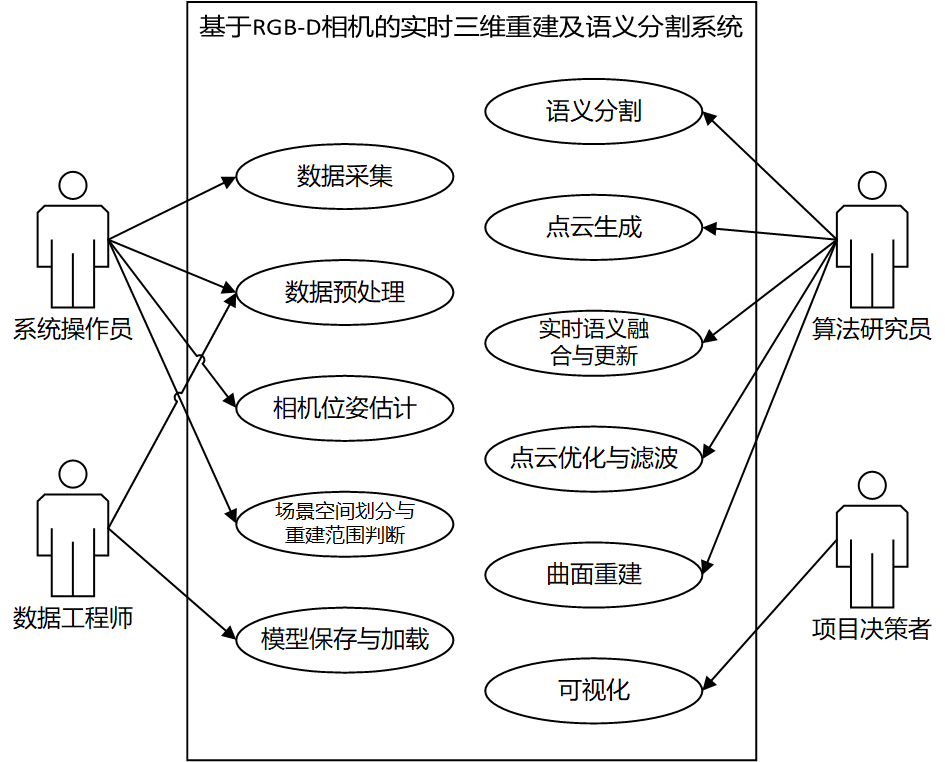
\includegraphics[width=0.9\textwidth]{figures/uml/case_all.png}
	\caption{系统功能用例图}
	\note{注:系统操作员、数据工程师、算法研究院和项目决策者各自承担不同的工作职责,使用系统的不同功能模块。}
	\label{fig:case_all}
\end{figure}

\par 如图\ref{fig:case_all}所示,设计一个基于RGB-D相机的实时三维重建及语义分割系统,需要考虑以下功能性需求:

\begin{enumerate}
	\item{数据采集}
	\par 如图\ref{fig:case1}所示,为了成功获取RGB-D相机的RGB图像和深度图像,系统需要与相机的硬件接口进行通信,这涉及到使用相机制造商提供的SDK。
	SDK包含一系列代码库和驱动程序,功能包括设置图像分辨率、调整曝光和焦距等特性。
	系统需要对这些功能进行封装,以便于后续步骤调用。

	\begin{figure}[htb]
		\centering
		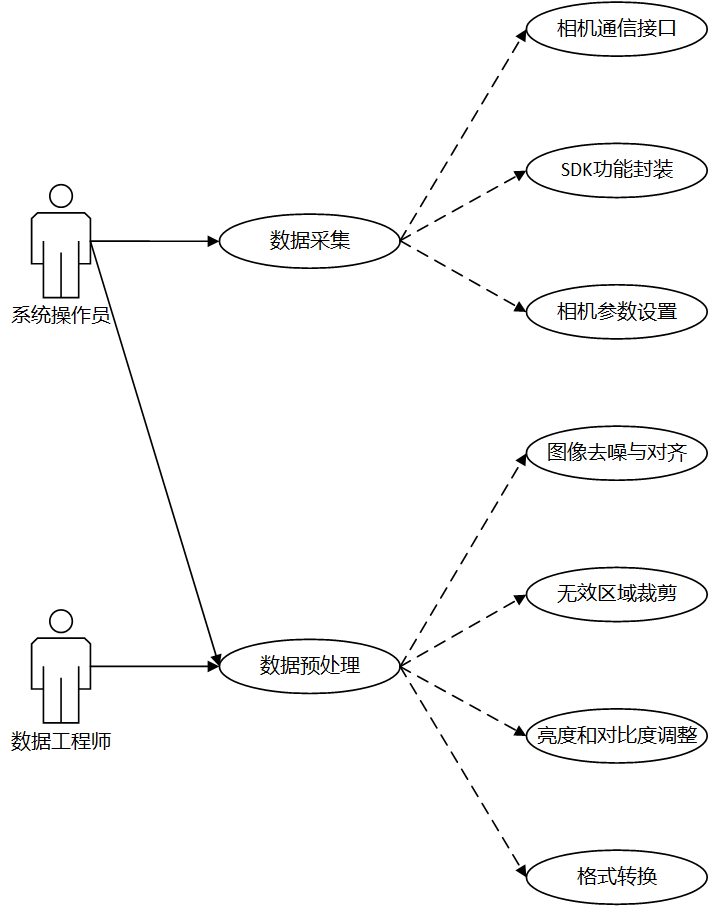
\includegraphics[width=0.618\textwidth]{figures/uml/case1.png}
		\caption{数据采集、数据预处理功能用例图}
		\label{fig:case1}
	\end{figure}

	\item{数据预处理}
	\par 从RGB-D相机获取数据后,需要对RGB图像和深度图像进行预处理,以提高后续步骤的准确性和效率,用例图如图\ref{fig:case1}所示。
	预处理首先包括图像去噪,用于提高图像的清晰度,减少图像噪声。
	其次,对图像进行格式转换,将图像格式转换为系统所需的格式,便于后续的计算和处理。
	第三,深度图像与RGB图像的对齐,这可以确保RGB图像和深度图像之间的一致性,使得每个像素点都具有正确的深度和RGB信息。
	第四,裁剪图像中的无效区域,如相机未能正确捕获的区域或视场之外的区域。
	最后,亮度和对比度的调整可以提高图像的可识别性和图像质量。

	\item{语义分割}
	\par 将RGB图像中的每个像素分类为不同的标签,如人、汽车、建筑物等。这通常通过深度学习方法
	完成,如全卷积网络(Fully Convolutional Network,FCN)、SegNet或DeepLab等。这些模型在大量带标签的数据集上进行了训练,
	可以用于预测新的图像中像素的语义标签,用例图如图\ref{fig:case2}所示。

	\item{相机位姿估计}
	\par 三维重建需要根据连续的RGB图像和深度图像计算相机的位姿矩阵,如图\ref{fig:case2}所示。
	这可以使用2D-2D位姿估计方法完成。典型的方法包括特征点法和直接法。
	其中,特征点法先提取图像的关键点,然后通过匹配关键点估计位姿;直接法则通过直接最小化像素间的光度误差估计位姿。

	\begin{figure}[htb]
		\centering
		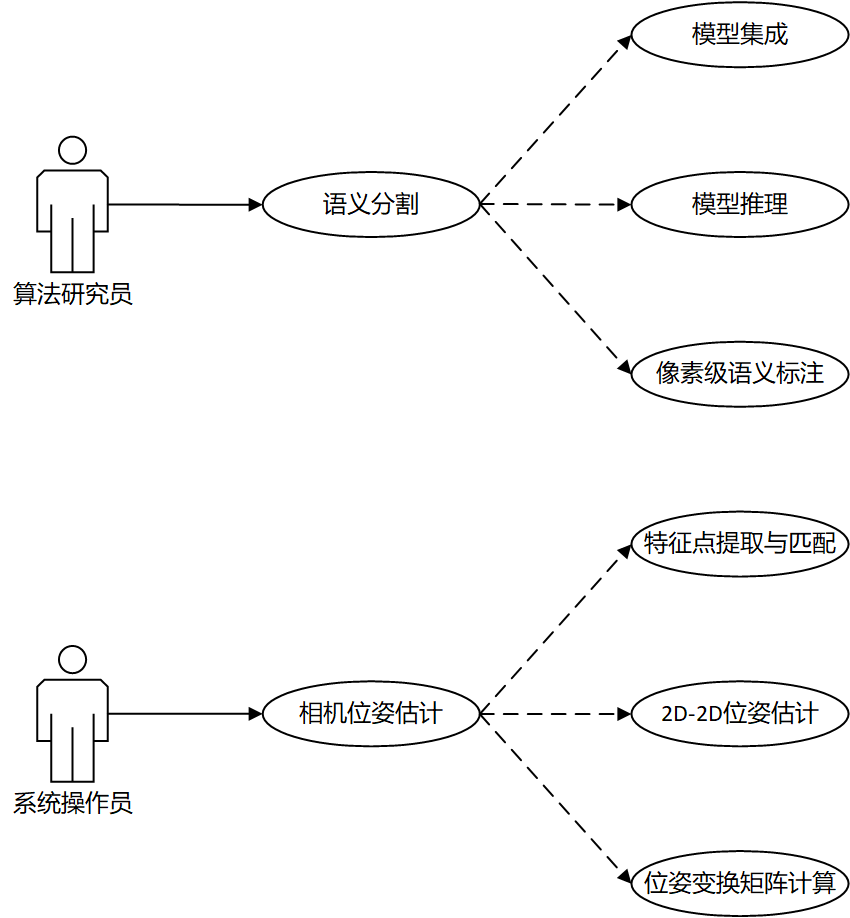
\includegraphics[width=0.618\textwidth]{figures/uml/case2.png}
		\caption{语义分割、相机位姿估计功能用例图}
		\label{fig:case2}
	\end{figure}

	\item{场景空间划分与重建范围判断}
	\par 由于内存的制约,若重建场景过大,则需要在场景空间中划分子区域,以便在有限的资源下进
	行重建,用例图如图\ref{fig:case3}所示。其中,场景空间划分将整个场景空间分成多个子区域,每个子区域具有一定的尺寸。这可以
	通过将空间划分为若干网格(如Spatial Grid)或者采用自适应的空间划分方法(如 Octree 数据结
	构)实现。重建范围判断应根据相机位姿矩阵,判断新的待重建空间是否超出了范围。如果超出
	范围,则先将GPU中的点云数据拷贝回CPU的点云数组中,根据所在网格保存为数据文件,然后读取
	新的网格中的模型进行增量式重建。

	\item{模型保存与加载}
	\par 系统需要能够灵活地导入和导出三维点云模型,便于与其他软件或设备兼容。如图\ref{fig:case3}所示,系统应使用主流
	的点云模型文件格式(如PLY、OBJ、PCD等),并能读取模型的几何信息、RGB信息和语义信息。在导入过程
	中还涉及模型格式转换、缩放、旋转、平移等操作,以确保导入模型信息与已当前模型保持一致。
	此外,系统需要能够在已有模型的基础上添加新的信息,与现有模型进行融合和更新。

	\begin{figure}[htb]
		\centering
		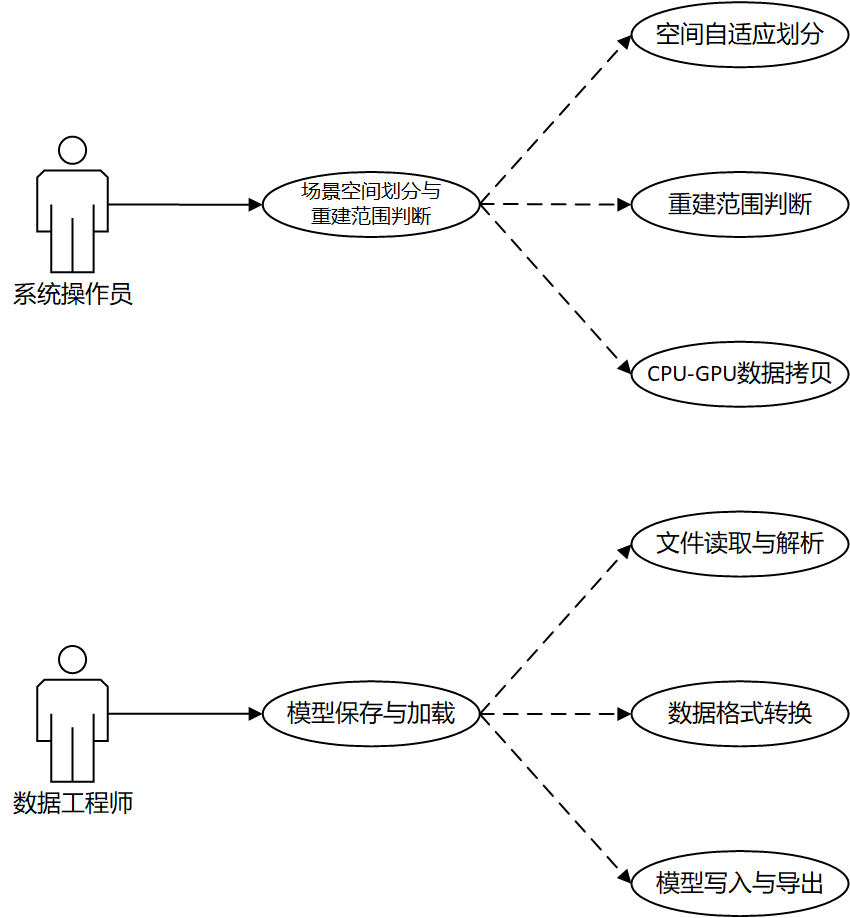
\includegraphics[width=0.618\textwidth]{figures/uml/case3.png}
		\caption{场景空间划分与重建范围判断、模型保存与加载功能用例图}
		\label{fig:case3}
	\end{figure}

	\par 同样,系统需要能够将重建的点云模型导出为常用文件格式,以便在其他软件或设备上使用。
	导出的模型可应用于CAD软件编辑、3D打印等场景。同时,应确保语义信息与模型一起导出,便于进一步分析和处理。

	\par 通过实现灵活的模型导入导出功能,系统能够满足不同应用需求,提高工作效率和便利性。

	\item{点云生成}
	\par 根据RGB图像、深度图像和相机位姿实时生成点云数据,将每个像素的RGB信息与其对应的三
	维坐标相关联。常用的方法有 TSDF、Structure from Motion(SfM)\cite{schonberger2016structure}以及Multi-View Stereo(MVS)\cite{furukawa2015multi}等。
	这些方法可以实现高效且准确的点云生成,为后续的语义融合提供几何模型基础。此外,可以利用GPU加速
	计算和多线程技术,进一步提高系统的性能。用例图如图\ref{fig:case4}所示。

	\begin{figure}[htb]
		\centering
		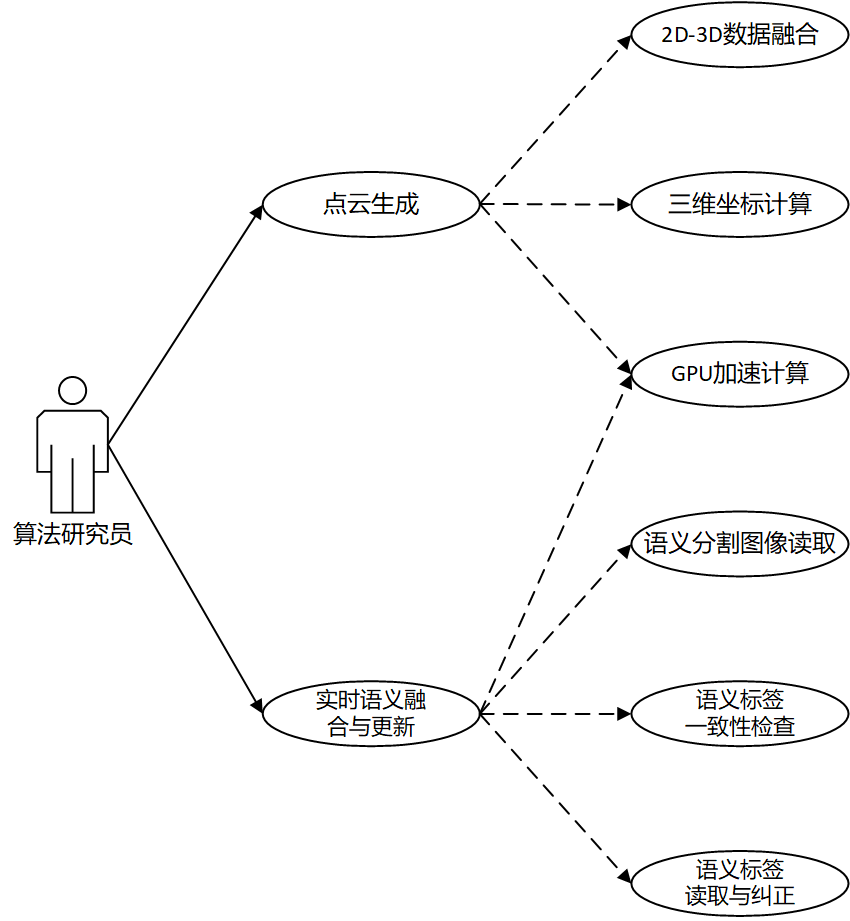
\includegraphics[width=0.618\textwidth]{figures/uml/case4.png}
		\caption{点云生成、实时语义融合与更新功能用例图}
		\label{fig:case4}
	\end{figure}

	\item{实时语义融合与更新}
	\par 根据语义分割图像,实时更新点云数据中的类别标签。系统需要在获取新的语义分割图像后,
	立即对点云数据进行语义融合与更新,这样有助于提高系统的交互性和用户体验。为了保证实时性,
	可以使用高效的算法实现,如线性分配方法(如匈牙利算法\cite{hungarian}、条件随机场等)\cite{zeng20163dmatch,online_panoptic_3d,panopticfusion,voxblox}。
	这些算法可以在较短的时间内对点云的语义信息进行一致性检查和纠正,确保生成的三维模型在几何和语义上保持一致。用例图如图\ref{fig:case4}所示。

	\item{点云优化与滤波}
	\par 对融合后的点云进行优化和滤波处理,以提高模型质量和精度,如图\ref{fig:case5}所示,包括去噪(统计滤波、高斯滤
	波或基于局部密度的滤波)、下采样(八叉树结构、VoxelGrid滤波或随机下采样等)以及法线估计
	等操作。

	\begin{figure}[htb]
		\centering
		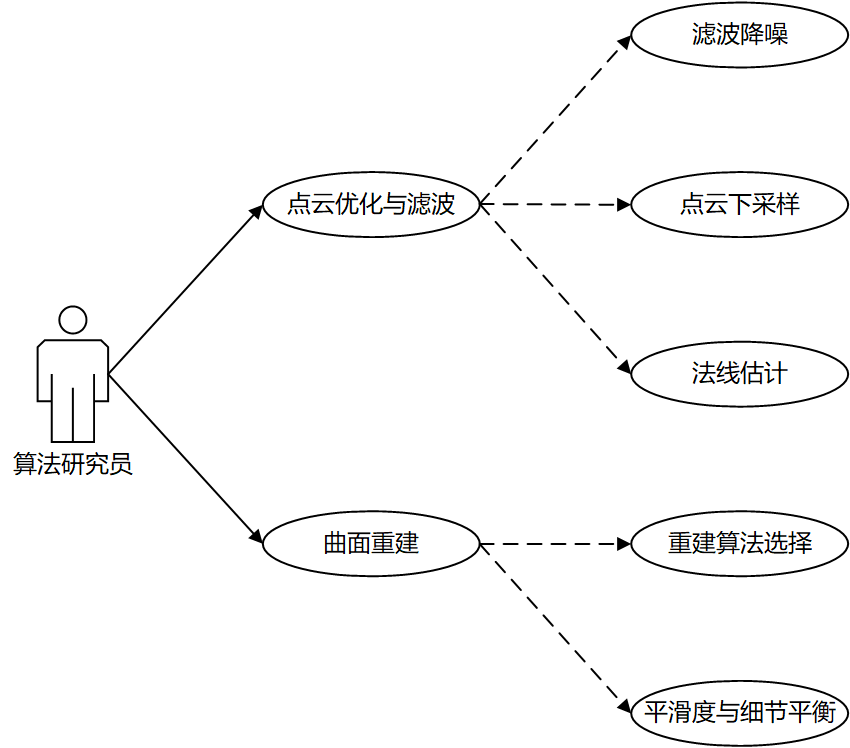
\includegraphics[width=0.618\textwidth]{figures/uml/case5.png}
		\caption{点云优化与滤波、曲面重建功能用例图}
		\label{fig:case5}
	\end{figure}

	\item{曲面重建(可选)}
	\par 如果需要从点云生成更连续的三维表面模型,可以使用曲面重建算法,例如贪婪投影三角化、
	泊松重建、球形重建等,以生成更连续、平滑的三维模型,使其适用于各种应用,如动画、游戏开发
	和虚拟现实。用例图如图\ref{fig:case5}所示。

	\item{可视化}
	\par 提供实时的图形用户界面,以便查看和分析重建的三维模型。可以使用现有的可视化图形库,如PCL Visualizer\cite{pcl}、Open3D Visualizer\cite{open3d}等,
	也可以基于OpenGL或Vulkan等图形库开发自定义的界面。图形用户界面可以显示点云生成、语义融合以及相机位姿变换的动画。
	此外,界面应具备用户友好的交互功能,例如缩放、旋转和平移视图,以便用户可以从不同角度和距离观察三维模型。用例图如图\ref{fig:case6}所示。

	\begin{figure}[htb]
		\centering
		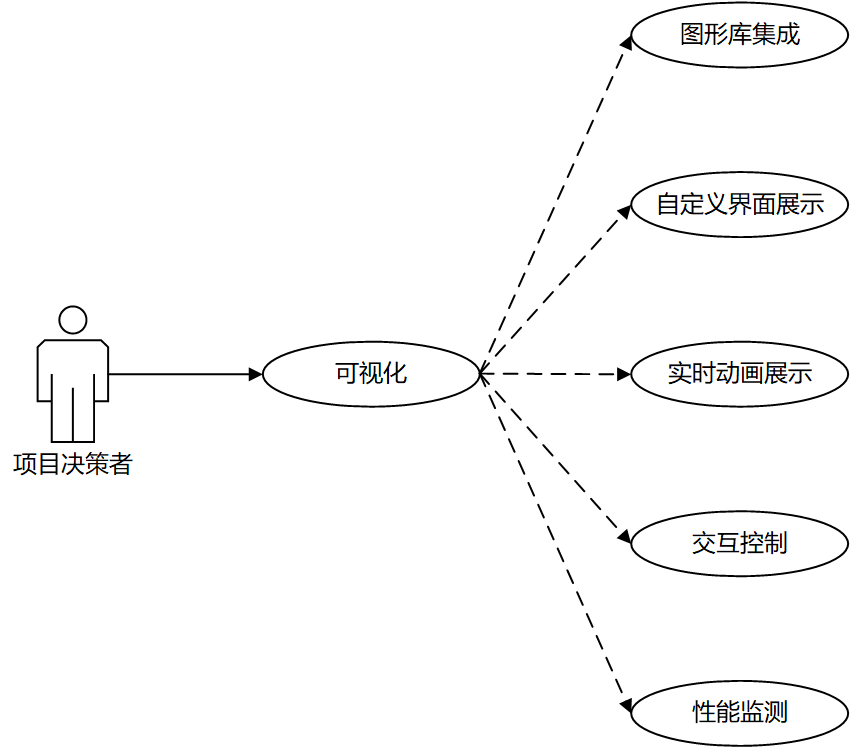
\includegraphics[width=0.618\textwidth]{figures/uml/case6.png}
		\caption{可视化功能用例图}
		\label{fig:case6}
	\end{figure}

	\par 通过实时可视化点云生成与语义融合的过程,用户和开发者可以更好地了解系统的性能和输出
	模型的质量,以便在需要时进行调整和优化。

\end{enumerate}

\par 这些功能性需求根据具体实现和应用需求而有所不同。在系统开发过程中,需要根据项目需
求和性能要求选择合适的算法和技术。

\section{非功能性需求}
\par 除了功能性需求外,还需要考虑以下非功能性需求,并且为每个需求设定具体的量化指标:

\begin{enumerate}
	\item{精度}
	\par 系统应能够准确地重建三维模型和进行语义分割。这包括从RGB-D数据中提取精确的几何信息
	、保持颜色一致性以及准确地识别和分类物体。为提高精度,需要采用先进的算法、机器学习技术以
	及高质量的数据。为适用室内重建,系统生成的点云模型与对应的实际物体的距离误差不应超过3 cm,语义重建正确率应大于50\%。

	\item{速度}
	\par 关注系统的重建速度,确保在有限时间内完成三维重建和语义分割任务,涉及选择合适的硬
	件、算法优化、并行计算等策略。为实现实时重建,每帧读取及预处理时间应小于5 ms,重建时间应
	小于 30 ms,总帧率应大于 30 帧/秒。

	\item{适应性}
	\par 系统需要能够适应不同场景和环境,如室内外、光线变化等情况。系统应在室内外光线变化范
	围内实现稳定运行,并且能够处理80\%以上的预设场景。

	% \item{可扩展性}
	% \par 系统应具备良好的可扩展性,以便在需要时添加新功能(如实例分割)或适应新的应用场景(
	% 如混合现实、游戏引擎)。这通常需要使用模块化设计、面向对象编程等技术。系统添加新功能或适
	% 应新应用场景的时间成本不超过一周。

	% \item{可维护性}
	% \par 为确保系统的可维护性,需要编写清晰、结构良好且注释充分的代码,代码注释覆盖率不低于
	% 80\%。此外,应提供涵盖所有功能模块及接口的文档和开发指南,这有助于其他开发者理解和维护系
	% 统。

	\item{可移植性}
	\par 系统应具备一定的可移植性,以便在不同平台和操作系统上运行。系统应支持Windows、Linux
	等多个主流操作系统。这需要使用跨平台的编程语言和库,遵循通用的编码规范。

	\item{系统稳定性}
	\par 考虑系统在各种环境和操作条件下的稳定性。需要处理异常情况,例如数据丢失、相机故障等
	,以确保系统的稳定运行。在各种环境和操作条件下,系统正常运行时间占比不低于95\%。

	\item{易用性}
	\par 系统应当具备友好的图形用户界面和操作流程,便于用户快速上手和使用。

	\item{资源占用}
	\par 考虑系统对计算资源的占用,优化系统以降低资源占用,提高整体性能。系统运行过程中CPU使
	用率不超过 80\%,内存占用不超过 50\%。

\end{enumerate}

\par 系统设计需要权衡这些非功能性需求与系统性能、开发时间和成本之间的关系。同时,与上下游子系
统的开发人员保持良好的沟通,确保需求得到充分理解和满足。最后,在开发过程中,定期评估进度和质量,对
需求进行调整,以实现系统开发目标。
\section{本章小结}
\par 本章对基于 RGB-D 相机的实时三维重建及语义分割系统进行了需求分析。
首先明确了系统的功能性需求,这包括数据采集、数据预处理、语义分割、相机位姿估计、场景划分与重建范围判断、模型保存与加载、点云生成、实时语义融合与更新、点云优化与滤波、曲面重建以及可视化等多个方面。
同时,也考虑到了非功能性需求,比如精度、速度、适应性、可扩展性、可维护性、可移植性、系统稳定性、用户体验和资源占用等。
这些需求为系统的设计和实现提供了方向,保证了系统的实用性和效率。
